\documentclass[letterpaper]{article} % DO NOT CHANGE THIS
\usepackage[submission]{aaai2026}  % DO NOT CHANGE THIS
\usepackage{times}  % DO NOT CHANGE THIS
\usepackage{helvet}  % DO NOT CHANGE THIS
\usepackage{courier}  % DO NOT CHANGE THIS
\usepackage[hyphens]{url}  % DO NOT CHANGE THIS
\usepackage{graphicx} % DO NOT CHANGE THIS
\urlstyle{rm} % DO NOT CHANGE THIS
\def\UrlFont{\rm}  % DO NOT CHANGE THIS
\usepackage{natbib}  % DO NOT CHANGE THIS AND DO NOT ADD ANY OPTIONS TO IT
\usepackage{caption} % DO NOT CHANGE THIS AND DO NOT ADD ANY OPTIONS TO IT
\frenchspacing  % DO NOT CHANGE THIS
\setlength{\pdfpagewidth}{8.5in} % DO NOT CHANGE THIS
\setlength{\pdfpageheight}{11in} % DO NOT CHANGE THIS
%
% These are recommended to typeset algorithms but not required. See the subsubsection on algorithms. Remove them if you don't have algorithms in your paper.
\usepackage{algorithm}
\usepackage{algorithmic}

\usepackage{pifont} %182/183/184
\usepackage{subcaption}
\usepackage{verbatim}
\usepackage{graphicx}
\usepackage{multirow}
\usepackage{xspace}
\usepackage{amsfonts,amssymb} 
\usepackage{microtype}
\usepackage{amsmath}
\usepackage{amsthm}
\usepackage{booktabs}
%\usepackage{subfigure}
\usepackage{times}
\usepackage{latexsym}
\usepackage{color}
\usepackage[dvipsnames, table]{xcolor}
\usepackage{soul}
\usepackage{verbatim}
\usepackage{multirow}
\usepackage{xspace}
\usepackage{amsfonts,amssymb} 
\usepackage{microtype}
%\usepackage{subfigure}
\usepackage{times}
\usepackage{latexsym}
\usepackage{color}
\usepackage[dvipsnames, table]{xcolor}
\usepackage{soul}
\usepackage{colortbl}
\usepackage{booktabs,makecell, multirow, tabularx}
\usepackage{adjustbox}
\usepackage{xcolor}
\usepackage{listings}
\usepackage{amsmath}

\usepackage{booktabs}
\usepackage{amssymb}
\usepackage{bbding}
\usepackage{pifont}
\usepackage{wasysym}
\usepackage{utfsym}
\usepackage{fontawesome}
\definecolor{special_yellow}{rgb}{1, 0.7412, 0.0353}
\definecolor{special_green}{rgb}{0.4314, 0.6392, 0.596}
\newcommand{\tick}{\textcolor{green}{\ding{51}}}  
\newcommand{\cross}{\textcolor{red}{\ding{55}}} 
\newcommand{\hollowstar}{\text{\ding{73}}}
\newcommand{\solidstar}{\text{\ding{72}}}

\usepackage{mdframed}
\begin{document}


\begin{table*}[h!]
\centering
\caption{Performance of models on OmniBench. For each capability, we use the CR metric on test tasks for quantification.}
\resizebox{\textwidth}{!}{%
\begin{tabular}{lcccccccccccc}
 \toprule 
  \multirow{2}{*}{} & \multicolumn{2}{c}{\textbf{\makecell{Overall}}} & \multicolumn{2}{c}{\textbf{\makecell{Planning}}} & \multicolumn{2}{c}{\textbf{\makecell{Decision-making}}} & \multicolumn{2}{c}{\textbf{\makecell{Instruction\\Understanding}}} & \multicolumn{2}{c}{\textbf{\makecell{Long Context}}} & \multicolumn{2}{c}{\textbf{\makecell{Generalist\\Knowledge}}} \\ \cline{2-13}
  & $CR$ & $LC$ & $PP$ & $LRP$ & $CDDK$ & $SDK$ & $SI$ & $DI$ & $LSR$ & $LIF$ & $DSK$ & $CDK$ \\ \midrule
 Human & 80.1 & 92.8 & 80.1 & 76.9 & 91.9 & 93.0 & 69.1 & 72.1 & 79.5 & 66.1 & 89.4 & 71.5 \\ \midrule
 \rowcolor{orange!20}
 \multicolumn{13}{c}{\textit{Open-source Multimodal Large Language Models~(A11Y+Screenshot)}} \\
 Qwen2-VL-7B~\cite{qwen2vl} & 14.8 & 9.0 & 15.5 & 13.5 & 16.5 & 17.8 & 14.1 & 13.8 & 14.7 & 12.4 & 15.8 & 13.8 \\
 InternVL2-8B~\cite{internvl} & 14.2 & 13.0 & 15.0 & 13.5 & 16.2 & 16.9 & 12.1 & 12.9 & 15.8 & 11.7 & 15.8 & 12.4 \\
 InternVL2.5-8B~\cite{internvl} & 17.4 & 18.8 & 18.2 & 16.7 & 19.6 & 21.5 & 16.4 & 15.3 & 15.8 & 15.4 & 19.0 & 16.3 \\ 
  \rowcolor{blue!20}
 \multicolumn{13}{c}{\textit{Closed-source Multimodal Large Language Models~(A11Y+Screenshot)}} \\
Qwen-VL-Max~\cite{qwenvl} & 18.4 & 23.3 & 18.7 & 19.4 & 19.6 & 23.3 & 15.0 & 16.7 & 18.3 & 16.1 & 19.6 & 17.3 \\ 
Gemini-2.0-Flash & 25.9 & \underline{38.0} & 24.8 & 24.6 & 31.5 & \underline{33.2} & 22.5 & 22.5 & 25.7 & 21.9 & 27.8 & \underline{24.8} \\ 
Claude-3.5-Sonnet & \underline{27.6} & 35.0 & \underline{30.5} & \underline{24.7} & \underline{32.0} & 31.3 & \underline{24.5} & \underline{25.0} & \underline{26.6} & \underline{23.5} & \underline{33.4} & 24.5 \\ 
GPT-4o~\cite{gpt} & \textbf{38.7} & \textbf{49.0} & \textbf{38.4} & \textbf{37.8} & \textbf{43.2} & \textbf{49.4} & \textbf{30.6} & \textbf{35.5} & \textbf{42.7} & \textbf{32.2} & \textbf{43.2} & \textbf{34.2} \\  \midrule
  \rowcolor{green!20} 
 \multicolumn{13}{c}{\textit{Visual Digital Agents~(Screenshot)}} \\
 Aguvis-7B~\cite{aguvis} & 22.9 & {27.1} & 21.2 & 23.5 & 25.5 & 28.1 & 20.2 & 20.0 & 22.8 & 20.1 & 26.3 & 21.6 \\
 OS-Atlas-Pro-4B~\cite{os-atlas} & {19.1} & 23.9 & 20.6 & 17.6 & 22.9 & 23.6 & 15.0 & 17.7 & 18.7 & 15.9 & 22.0 & 16.8 \\
 ShowUI-2B\textsuperscript{*}~\cite{showui} & 23.2 & 24.6 & 23.2 & 23.1 & 26.3 & 26.6 & 21.5 & 20.3 & 24.7 & 20.4 & 24.8 & 20.7 \\
 OS-Atlas-Base-4B\textsuperscript{*}~\cite{os-atlas} & 22.2 & 23.8 & 23.2 & 21.9 & 26.2 & 25.6 & 19.4 & 19.5 & 23.5 & 20.0 & 23.4 & 19.3 \\
 UGround-V1-7B\textsuperscript{*}~\cite{uground} & 25.0 & 26.3 & \underline{25.7} & {25.1} & 30.6 & {31.4} & 21.5 & 21.3 & {24.8} & 21.3 & 27.2 & {21.5} \\
  \rowcolor{purple!20}
 \multicolumn{13}{c}{\textit{Supervised Fine-Tuning Agents~(Screenshot)}} \\
  Omni-OS-Atlas-Base-4B~(Ours) & \underline{29.7} & \underline{30.1} & 24.2 & \textbf{33.0} & \underline{34.9} & \underline{35.3} & \textbf{28.7} & \underline{24.2} & \underline{27.9} & \underline{26.5} & \underline{33.8} & \textbf{28.2} \\
 Omni-UGround-V1-7B~(Ours)  & \textbf{34.4} & \textbf{37.4} & \textbf{33.2} & \underline{31.3} & \textbf{43.1} & \textbf{42.4} & \underline{21.9} & \textbf{35.0} & \textbf{40.3} & \textbf{31.7} & \textbf{36.7} & \underline{27.6} \\
 
\bottomrule
\end{tabular}
}
\label{maintable}
\vspace{-7mm}
\end{table*}


\begin{table*}[h!]
\vspace{-6mm}
\caption{Comparison of virtual agent benchmarks across environment, task, and evaluation dimensions. Unlike previous benchmarks, OmniBench features automatic task composition, five-dimensional task complexity, and a 10-capability evaluation framework.}
\centering
\resizebox{\textwidth}{!}{%
\begin{tabular}{l|ccc|cccccccc|cccc}
\toprule
\multirow{2}{*}{} & \multicolumn{3}{c|}{\textbf{Environment}} & \multicolumn{8}{c|}{\textbf{Task}} & \multicolumn{4}{c}{\textbf{Evaluation}} \\ \cline{2-16}
& \textbf{\makecell{Interactive}} & \textbf{\makecell{Real-World}} & \textbf{\makecell{Platform}} & \textbf{\makecell{\# Instance}} & \textbf{\makecell{\# Compl.\\Dimen.}} & \textbf{\makecell{Dyna.\\Scale}} & \textbf{Intent} & \textbf{\# Scenario} & \textbf{\makecell{Demo.\\Traj.}} & \textbf{Construction} & \textbf{\makecell{Instruction\\Level}} & \textbf{\makecell{\# Cap.\\Dimen.}} & \textbf{\makecell{Eval.\\Level}} & \textbf{\makecell{\# Eval.\\Func.}} & \textbf{\makecell{Evaluation\\Strategy}} \\ \hline
 AitW~\cite{aitw} & \cross & \cross & 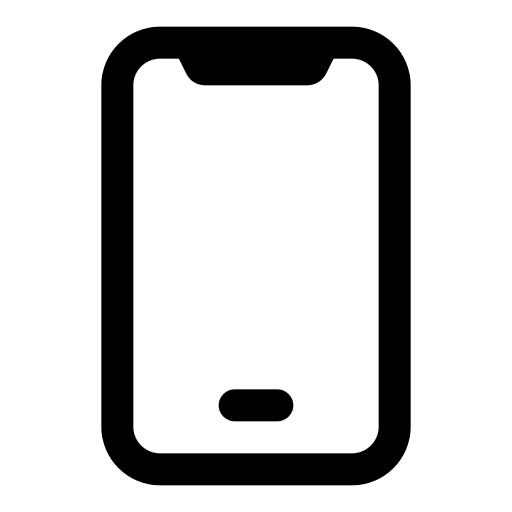
\includegraphics[width=0.4cm]{image/mobile.png} & 30378 & - & \cross & \cross & 5 & \tick & Manual Annotation & High \& Low & 1 & Task & - & Trajectory-based \\
 Mind2Web~\cite{mind2web} & \cross & \cross & 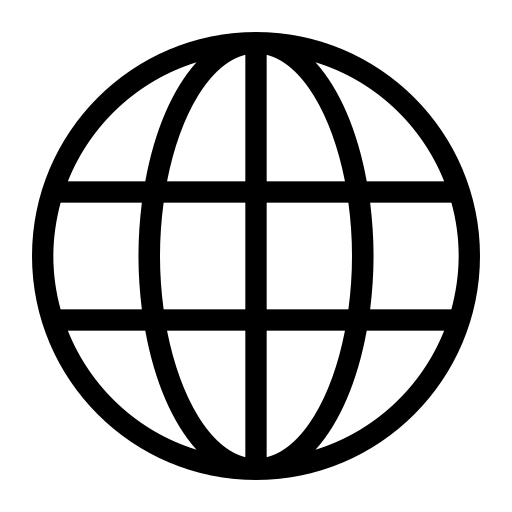
\includegraphics[width=0.4cm]{image/web.png} & 2350 & - & \cross & \cross & 5 & \tick & Manual Annotation & High & 1 & Task & - & Trajectory-based \\ 
 MoTIF~\cite{motif} & \cross & \cross & 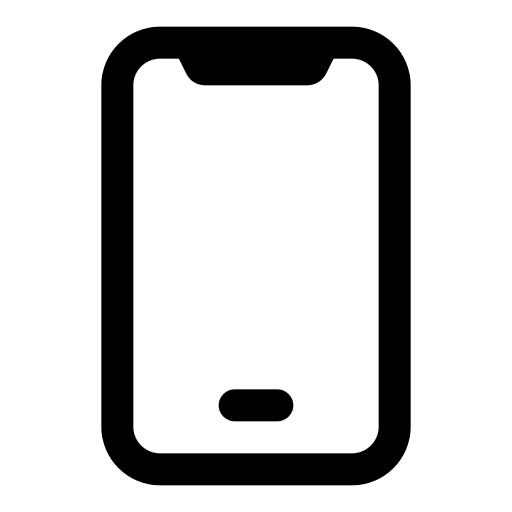
\includegraphics[width=0.4cm]{image/mobile.png} & 756 & - & \cross & \cross & - & \tick & Manual Annotation & High \& Low & 1 & Task & - & Trajectory-based \\
 OmniACT~\cite{omniact} & \cross & \cross & 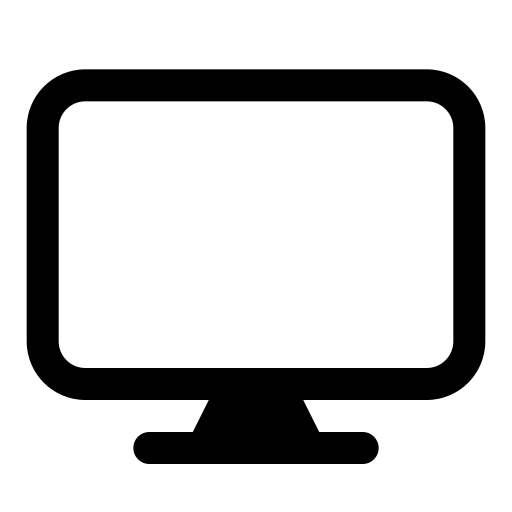
\includegraphics[width=0.4cm]{image/desktop.png} 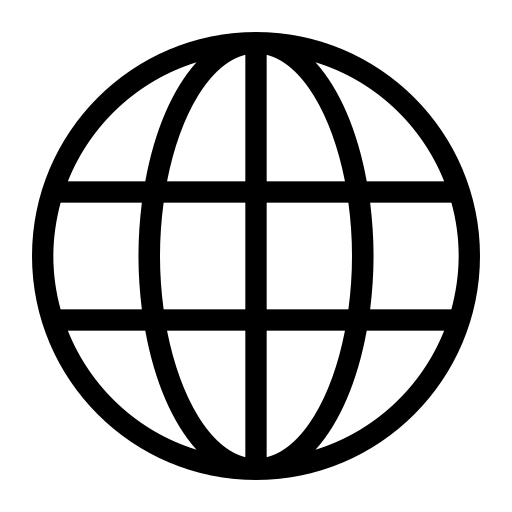
\includegraphics[width=0.4cm]{image/web.png} & 9802 & - & \cross & \cross & 6 & \tick & Manual Annotation & Low & 1 & Task & - & Trajectory-based \\
 GUI Odyssey~\cite{gui-odyssey} & \cross & \cross & 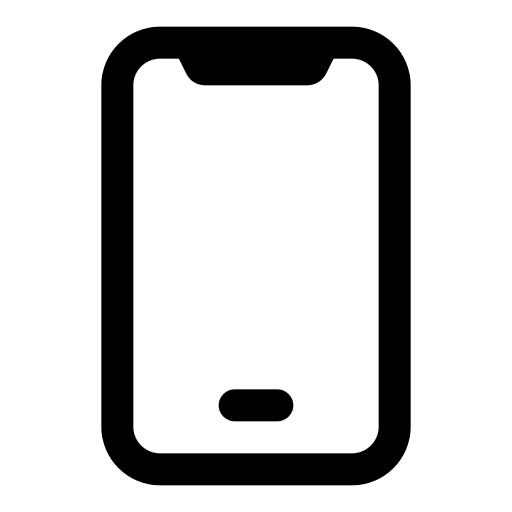
\includegraphics[width=0.4cm]{image/mobile.png} 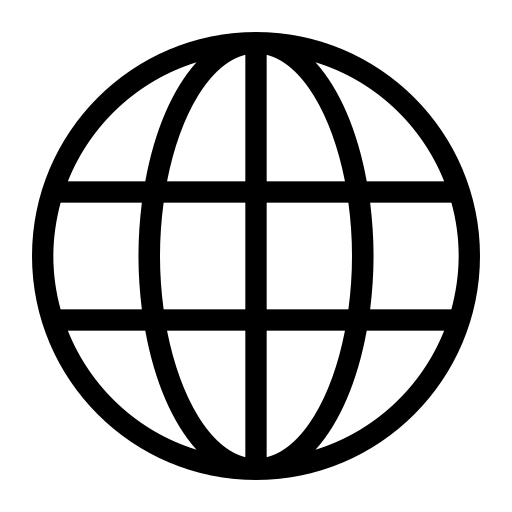
\includegraphics[width=0.4cm]{image/web.png} & 7735 & - & \cross & \cross & 6 & \tick & Manual Annotation & Low & 1 & Task & - & Trajectory-based \\ \hline
 WebArena~\cite{webarena} & \tick & \cross & 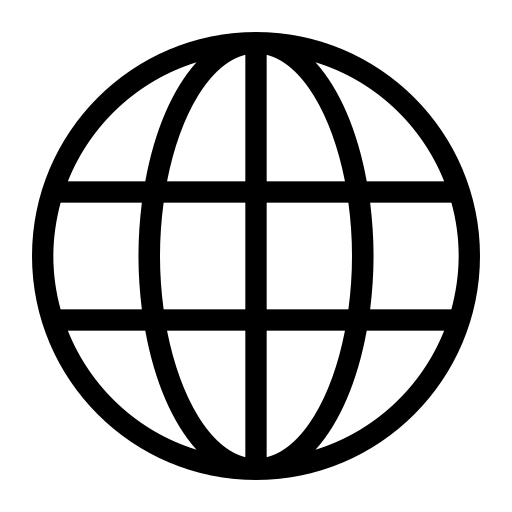
\includegraphics[width=0.4cm]{image/web.png} & 812 & - & \cross & \cross & 4 & \cross & Manual Annotation & Low & 1 & Task & 5 & Result-based \\
 VisualWebArena~\cite{visualwebarena} & \tick & \cross & 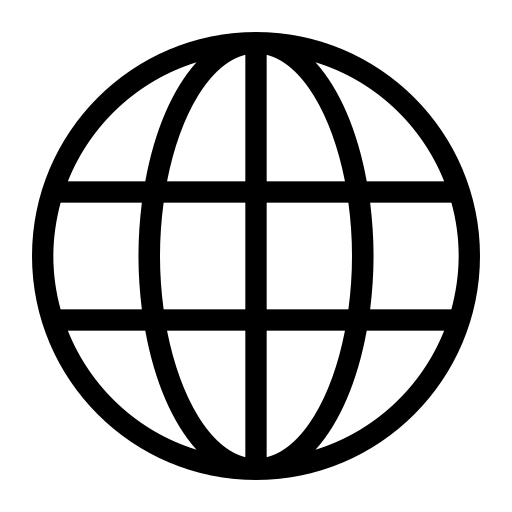
\includegraphics[width=0.4cm]{image/web.png} & 910 & 2 & \cross & \cross & 3 & \cross & Manual Annotation & Low & 1 & Task & 6 & Result-based \\ 
 OSWorld~\cite{osworld} & \tick & \tick & 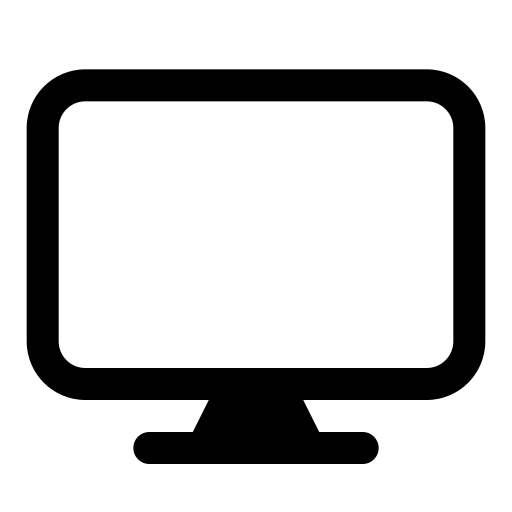
\includegraphics[width=0.4cm]{image/desktop.png} & 369 & - & \cross & \cross & 5 & \tick & Manual Annotation & Low & 1 & Task & 134 & Result-based \\
 Spider2-V~\cite{spider2-v} & \tick & \tick & 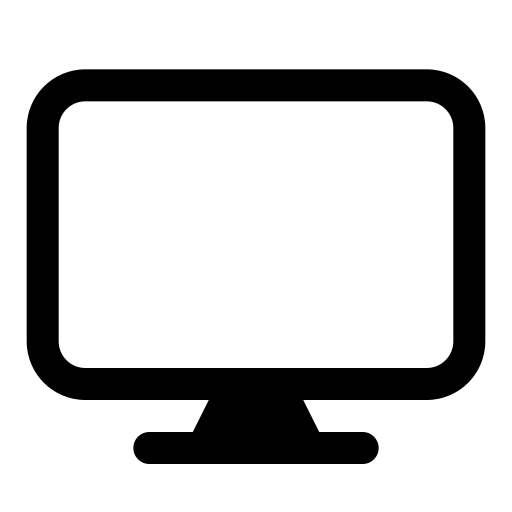
\includegraphics[width=0.4cm]{image/desktop.png} 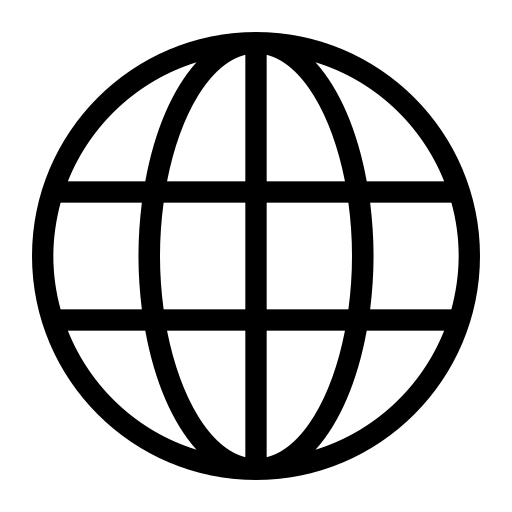
\includegraphics[width=0.4cm]{image/web.png} & 494 & 1 & \cross & \cross & 7 & \cross & Manual Annotation & High \& Low & 1 & Task & 151 & Result-based \\ 
 CRAB~\cite{crab} & \tick & \tick & 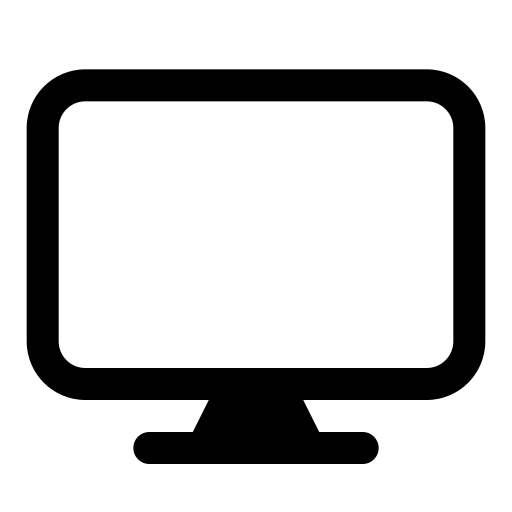
\includegraphics[width=0.4cm]{image/desktop.png} 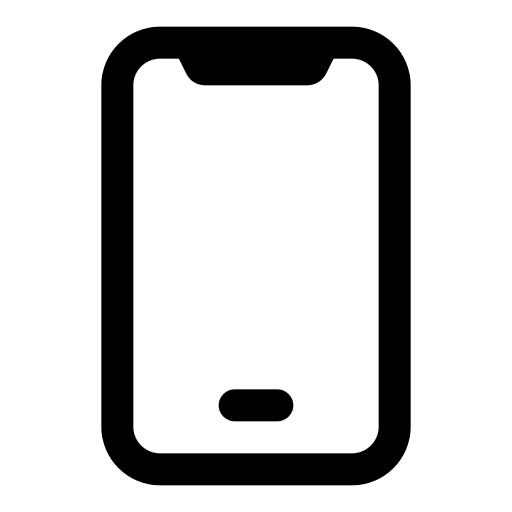
\includegraphics[width=0.4cm]{image/mobile.png} & 100 & - & \tick & \cross & - & \cross & Manual Composition & Low & 1 & Subtask & 59 & Graph-based \\ \hline
 OmniBench~(Ours) & \tick & \tick & 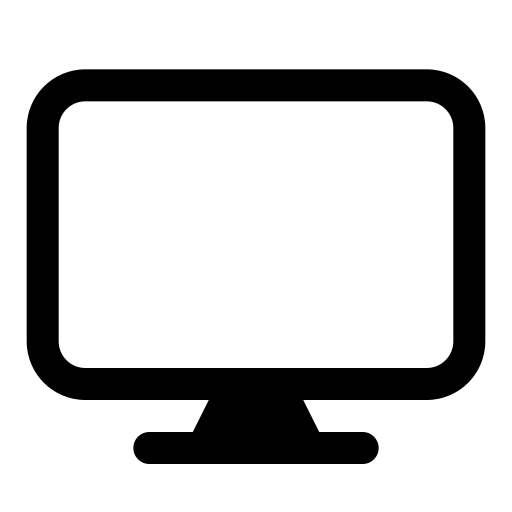
\includegraphics[width=0.4cm]{image/desktop.png} 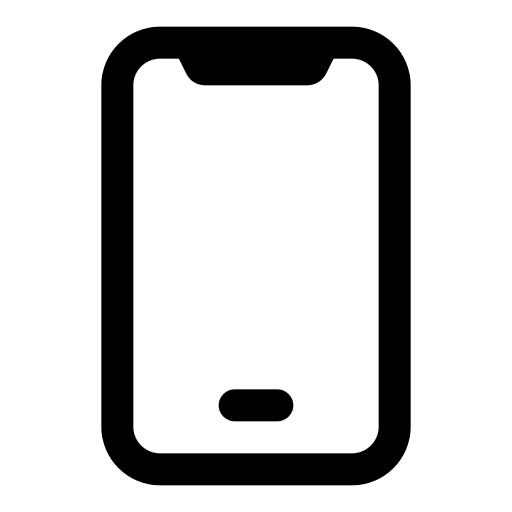
\includegraphics[width=0.4cm]{image/mobile.png} 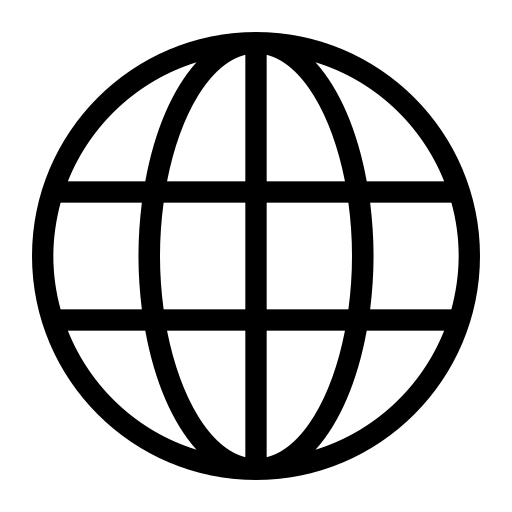
\includegraphics[width=0.4cm]{image/web.png} & 36076 & 5 & \tick & \tick & 20 & \tick & \makecell{Automatic Composition \\ \& Human Verification} & High \& Low & 10 & Subtask & 255 & Graph-based

 
 \\ \bottomrule
\end{tabular}%
}
\label{tab1}
\vspace{-6mm}
\end{table*}


\end{document}